\section{Movimiento de 2 cuerpos}

\subsection{Enunciado}

Se estudió el movimiento del objeto interestelar \textit{3I/ATLAS}, el cual atravesó el sistema solar siguiendo una trayectoria abierta alrededor del Sol. El objetivo fue modelar numéricamente su movimiento utilizando la ley de gravitación universal y datos aproximados obtenidos de información astronómica disponible públicamente.

Para el desarrollo del problema se consideraron:

\begin{itemize}
    \item Masa del Sol.
    \item Radio del Sol.
    \item Velocidad aproximada de 3I/ATLAS.
    \item Movimiento gravitacional de dos cuerpos.
\end{itemize}

El sistema se simplificó considerando únicamente la interacción gravitacional entre el Sol y el objeto interestelar.

\subsection{Modelo físico}

La fuerza gravitacional entre el Sol y el objeto se modeló mediante la ley de gravitación universal:

\begin{equation}
    \vec{F} = - \frac{GMm}{r^3}\vec{r}
\end{equation}

donde:

\begin{itemize}
    \item $G$ es la constante de gravitación universal.
    \item $M$ es la masa del Sol.
    \item $m$ es la masa del objeto.
    \item $r$ es la distancia entre ambos cuerpos.
\end{itemize}

A partir de esta expresión se obtuvieron las aceleraciones en cada eje:

\begin{equation}
    a_x = -\frac{x}{(x^2+y^2)^{3/2}}
\end{equation}

\begin{equation}
    a_y = -\frac{y}{(x^2+y^2)^{3/2}}
\end{equation}

Estas ecuaciones fueron implementadas numéricamente en MATLAB para calcular la trayectoria del objeto alrededor del Sol.

\subsection{Normalización de unidades}

Con el objetivo de simplificar los cálculos numéricos, las distancias fueron expresadas en radios solares.

Se tomó:

\begin{equation}
    R_{\odot} = \SI{696350}{\kilo\meter}
\end{equation}

Por tanto:

\begin{equation}
    1 \text{ unidad} = 1 R_{\odot}
\end{equation}

Las velocidades obtenidas de información astronómica fueron inicialmente expresadas en $\si{\kilo\meter/\hour}$ y posteriormente convertidas a radios solares por hora dividiendo entre el radio solar.

Las componentes aproximadas de velocidad utilizadas fueron:

\begin{equation}
    v_x \approx \SI{62689}{\kilo\meter/\hour}
\end{equation}

\begin{equation}
    v_y \approx \SI{-211922}{\kilo\meter/\hour}
\end{equation}

Luego de la conversión:

\begin{equation}
    v_x \approx 0.090
\end{equation}

\begin{equation}
    v_y \approx -0.304
\end{equation}

Las posiciones iniciales también fueron expresadas en radios solares:

\begin{equation}
    x_0 = -458.33079
\end{equation}

\begin{equation}
    y_0 = 2665.95683
\end{equation}

Estos valores fueron estimados utilizando una hoja de cálculo para realizar conversiones y aproximaciones temporales hacia atrás desde el perihelio.

\subsection{Implementación numérica}

La trayectoria se calculó utilizando integración temporal mediante el método de Euler explícito.

La implementación utilizada se muestra en el Código \ref{lst:atlas}.

\begin{listing}[H]
\inputminted[
    linenos,
    frame=lines,
    fontsize=\small
]{matlab}{code/problem02.m}
\caption{Simulación numérica de la trayectoria de 3I/ATLAS.}
\label{lst:atlas}
\end{listing}

La simulación se realizó utilizando un tamaño de paso pequeño para reducir el error numérico durante la integración.

\subsection{Resultados}

La Figura \ref{fig:atlas} muestra la trayectoria obtenida para el objeto interestelar al pasar cerca del Sol.

\begin{figure}[H]
    \centering
    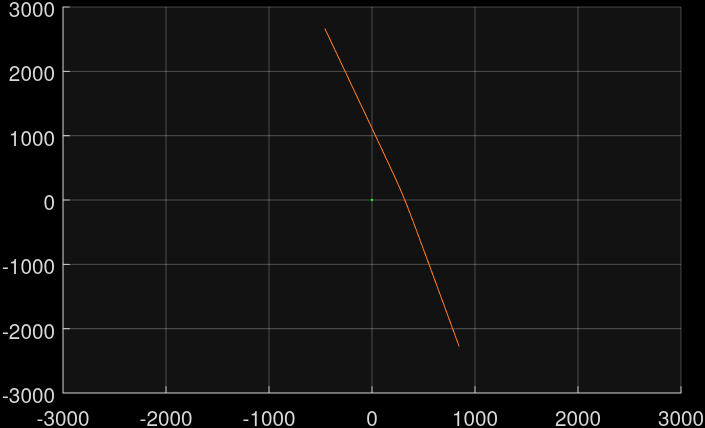
\includegraphics[width=0.75\textwidth]{images/problem02.png}
    \caption{Trayectoria aproximada de 3I/ATLAS alrededor del Sol.}
    \label{fig:atlas}
\end{figure}

En la figura se observa una trayectoria abierta característica de un objeto interestelar que no permanece ligado gravitacionalmente al Sol.

Debido a pequeñas variaciones decimales en las condiciones iniciales y en las conversiones realizadas, la trayectoria puede desplazarse aproximadamente entre 10 y 20 radios solares. Sin embargo, el comportamiento general permanece consistente y conserva la forma hiperbólica esperada.

Asimismo, la gráfica presenta una trayectoria visualmente muy abierta. Esto ocurre porque el objeto posee una velocidad extremadamente alta y la gravedad solar únicamente desvía parcialmente su movimiento.

\subsection{Tipo de trayectoria}

La trayectoria obtenida corresponde a una órbita hiperbólica.

Una órbita hiperbólica ocurre cuando la energía mecánica total del sistema es positiva, es decir, cuando el objeto posee suficiente velocidad para escapar permanentemente de la atracción gravitacional del Sol.

La excentricidad orbital cumple:

\begin{equation}
    e > 1
\end{equation}

En el caso de 3I/ATLAS, los datos astronómicos indican una excentricidad aproximada:

\begin{equation}
    e \approx 6.3
\end{equation}

lo cual confirma que el objeto proviene del espacio interestelar y continuará alejándose del sistema solar después de su acercamiento al Sol.

\subsection{Conclusiones}

La simulación permitió modelar de manera aproximada el movimiento de un objeto interestelar utilizando el problema gravitacional de dos cuerpos.

Los resultados obtenidos muestran una trayectoria hiperbólica abierta, coherente con las observaciones astronómicas reportadas para 3I/ATLAS.

Además, se verificó que pequeñas variaciones numéricas en las condiciones iniciales producen desplazamientos apreciables en la trayectoria, lo cual evidencia la sensibilidad del sistema a errores de redondeo y aproximación durante las conversiones numéricas.
